\documentclass{article}

% Basic packages
\usepackage{amsmath}
\usepackage{amsthm}
\usepackage{amssymb}
\usepackage{geometry}
\usepackage{tcolorbox}
\usepackage{tikz}
\usepackage{pgfplots}

% TikZ libraries
\usetikzlibrary{3d}
\usetikzlibrary{arrows.meta}
\usetikzlibrary{graphs}

% Page setup
\geometry{a4paper, margin=1in}

% Theorem environments
\newtheorem{theorem}{Theorem}
\newtheorem{definition}{Definition}
\newtheorem{lemma}{Lemma}
\newtheorem{corollary}{Corollary}

\begin{document}

\title{Special Relativity and Blockchain Consensus}
\author{Kevin Ting Kai Kuo}
\date{\today}
\maketitle

\section{Introduction}
This note explores the intersection of special relativity and blockchain consensus mechanisms.

\section{Formal Mathematical Framework}

\begin{definition}[Minkowski Spacetime]
The spacetime manifold $(M, \eta)$ consists of:
\begin{align*}
    M &= \mathbb{R}^4 \\
    \eta(v, v) &= -c^2t^2 + x^2 + y^2 + z^2 \\
    ds^2 &= -c^2dt^2 + dx^2 + dy^2 + dz^2
\end{align*}
\end{definition}

\begin{definition}[Light Cone]
For event $p \in M$:
\begin{align*}
    C(p) &= \{q \in M : \eta(q-p, q-p) = 0\} \\
    J^+(p) &= \{q \in M : \eta(q-p, q-p) \leq 0, t_q > t_p\} \\
    J^-(p) &= \{q \in M : \eta(q-p, q-p) \leq 0, t_q < t_p\}
\end{align*}
\end{definition}

\begin{theorem}[Local Consensus Formation]
Let $\mathcal{N} = (V, E)$ be a network where:
\begin{align*}
    V &= \{n_i\}_{i=1}^N \text{ (nodes)} \\
    E &= \{(n_i, n_j) : d(n_i, n_j) \leq ct\} \\
    \mathcal{C}(t) &= \{n_i \in V : \forall n_j \in V, (n_i, n_j) \in E\}
\end{align*}
Then:
\[ \exists R > 0 : \forall t, \forall n_i, n_j \in \mathcal{C}(t), d(n_i, n_j) \leq R \]
\end{theorem}

\begin{proof}
Let $\mathcal{P} = \{p_i\}_{i=1}^N$ be events in $M$. Then:
\begin{align*}
    &(1)\ \forall p_i, p_j \in \mathcal{P}: \\
    &\quad p_j \in J^+(p_i) \iff -c^2(t_j-t_i)^2 + \|\vec{x}_j-\vec{x}_i\|^2 \leq 0 \\
    &(2)\ \text{For consensus at time } T: \\
    &\quad \forall i,j: \|\vec{x}_j-\vec{x}_i\| \leq cT \\
    &(3)\ \text{By triangle inequality}: \\
    &\quad \|\vec{x}_k-\vec{x}_i\| \leq \sum_{j=1}^{n-1} \|\vec{x}_{j+1}-\vec{x}_j\| \leq ncT
\end{align*}
Therefore, $R = ncT$ bounds the consensus region.
\end{proof}

\section{DAG Structure and Quantum Field Theory}

\begin{definition}[Causal DAG]
For events $\mathcal{P}$, define graph $G = (\mathcal{P}, E)$ where:
\[ E = \{(p_i, p_j) : p_j \in J^+(p_i)\} \]
\end{definition}

\begin{lemma}[DAG Properties]
For any $p_i, p_j, p_k \in \mathcal{P}$:
\begin{align*}
    &(1)\ p_j \in J^+(p_i) \implies p_i \notin J^+(p_j) \\
    &(2)\ p_j \in J^+(p_i) \land p_k \in J^+(p_j) \implies p_k \in J^+(p_i) \\
    &(3)\ \nexists \{p_1,...,p_n\} : p_1 \to p_2 \to ... \to p_n \to p_1
\end{align*}
\end{lemma}

\begin{definition}[TQFT Action]
For quantum field $\Phi$ on DAG $G$:
\begin{align*}
    S[\Phi] &= \sum_{(p_i \to p_j) \in E} f(\psi_i, \psi_j) \\
    f(\psi_i, \psi_j) &= \|\psi_j - U_{ij}\psi_i\|^2 \\
    U_{ij} &= \exp(-iH_{ij}\Delta t_{ij})
\end{align*}
where $H_{ij}$ is the interaction Hamiltonian.
\end{definition}

\begin{corollary}[Spacetime Arbitrage Condition]
For subgraphs $\mathcal{G}_1, \mathcal{G}_2$ with consensus times $T_1, T_2$:
\begin{align*}
    &\text{Arbitrage possible} \iff \\
    &\exists \Delta T = T_2 - T_1 > 0 : \\
    &\quad P(\text{success}|\Delta T) > \frac{C_{\text{transaction}}}{R_{\text{arbitrage}}}
\end{align*}
where $C_{\text{transaction}}$ is transaction cost and $R_{\text{arbitrage}}$ is potential return.
\end{corollary}

\section{Properties of Local Consensus under Light Speed Constraint}

\begin{theorem}[Local Consensus Formation]
In a spacetime grid governed by special relativity, assuming a distributed clock network where each clock exchanges information under the light speed constraint, consensus formation must satisfy locality conditions, meaning it can only be achieved within regions supported by light cones.
\end{theorem}

\begin{proof}
Consider a spacetime $(M, \eta)$ consisting of a 4-dimensional manifold $M$ and the Minkowski metric $\eta$, where $\eta(v, v) = -c^2t^2 + x^2 + y^2 + z^2$.

The light cone $C(p)$ of an event $p$ consists of all events $q$ satisfying $\eta(q-p,q-p)=0$, which can be divided into:
\begin{itemize}
    \item Future light cone $J^+(p)$: events $q$ in $p$'s future where $t_q > t_p$
    \item Past light cone $J^-(p)$: events $q$ in $p$'s past where $t_q < t_p$
\end{itemize}

Let the distributed clock network consist of nodes $N = \{n_i\}$, where information exchange between nodes cannot exceed the speed of light $c$. For any two events $p_i$ and $p_j$ at different nodes, $p_j$ must lie within the future light cone $J^+(p_i)$ to receive information.

Consensus formation requires all nodes to receive information from each other. However, due to the light speed constraint, consensus can only be achieved within a finite region inside the light cone. Nodes outside the light cone cannot participate in consensus, thus creating locality phenomena.
\end{proof}

\begin{figure}[h]
\centering
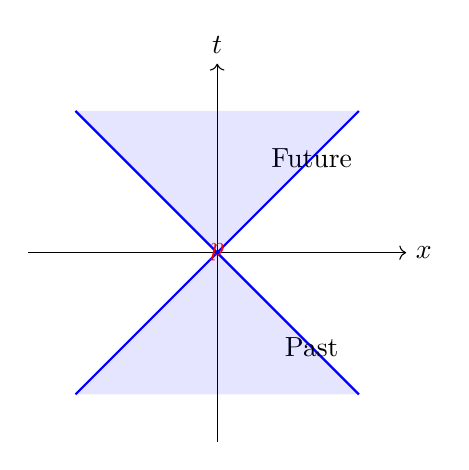
\begin{tikzpicture}[scale=1.2]
    % Axes
    \draw[->] (-2,0) -- (2,0) node[right] {$x$};
    \draw[->] (0,-2) -- (0,2) node[above] {$t$};
    
    % Light cone
    \draw[blue, thick] (-1.5,1.5) -- (0,0) -- (1.5,1.5);
    \draw[blue, thick] (-1.5,-1.5) -- (0,0) -- (1.5,-1.5);
    
    % Labels
    \node at (1,1) {Future};
    \node at (1,-1) {Past};
    \node[red] at (0,0) {$p$};
    
    % Fill light cone regions with different opacity
    \fill[blue,opacity=0.1] (-1.5,1.5) -- (0,0) -- (1.5,1.5);
    \fill[blue,opacity=0.1] (-1.5,-1.5) -- (0,0) -- (1.5,-1.5);
\end{tikzpicture}
\caption{Light cone structure in 2D spacetime showing future and past regions}
\label{fig:lightcone}
\end{figure}

\section{Mathematical Implications: Light Cone Structure and DAG}

\begin{corollary}[Light Cone Events Form a DAG]
In spacetime $(M, \eta)$, light cone events naturally form a Directed Acyclic Graph (DAG).
\end{corollary}

\begin{proof}
For any two events $p_i, p_j$, if $p_j \in J^+(p_i)$, we define a directed edge $p_i \to p_j$. This structure satisfies:
\begin{itemize}
    \item Directedness: If $p_i \to p_j$, then $p_j \not\to p_i$
    \item Acyclicity: A cycle $p_1 \to p_2 \to \dots \to p_k \to p_1$ would violate causality and thus cannot exist
\end{itemize}
\end{proof}

\begin{figure}[h]
\centering
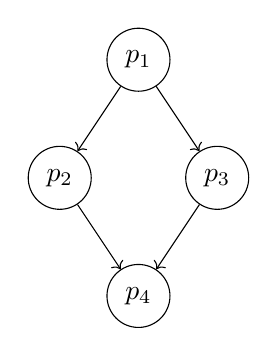
\begin{tikzpicture}[
    node distance=1.5cm,
    every node/.style={circle, draw, minimum size=0.8cm}
]
    % Nodes
    \node (1) at (0,0) {$p_1$};
    \node (2) at (-1,-1.5) {$p_2$};
    \node (3) at (1,-1.5) {$p_3$};
    \node (4) at (0,-3) {$p_4$};
    
    % Edges
    \draw[->] (1) -- (2);
    \draw[->] (1) -- (3);
    \draw[->] (2) -- (4);
    \draw[->] (3) -- (4);
\end{tikzpicture}
\caption{Example of a DAG formed by light cone events}
\label{fig:dag}
\end{figure}

\begin{corollary}[DAG-based TQFT]
Let $\mathcal{G}$ be a DAG formed by light cone events with nodes $\{p_i\}$, each having state $\psi_i$. The topological quantum field $\Phi$ has action:
\[ S[\Phi] = \sum_{(p_i \to p_j) \in \mathcal{G}} f(\psi_i, \psi_j) \]
where $f(\psi_i, \psi_j)$ represents node interactions.
\end{corollary}

\begin{lemma}[Spacetime Arbitrage]
In a large-scale blockchain network split into subgraphs $\mathcal{G}_1, \mathcal{G}_2, \dots, \mathcal{G}_m$, if consensus times $T_1$ and $T_2$ for subgraphs $\mathcal{G}_1$ and $\mathcal{G}_2$ satisfy $T_2 - T_1 > 0$, nodes can perform arbitrage operations exploiting this time difference, utilizing synchronization delays caused by light speed limitations.
\end{lemma}

\begin{corollary}[DAG-based TQFT Properties]
Let $\mathcal{G} = (\mathcal{P}, E)$ be a DAG formed by light cone events. The TQFT system satisfies:

1. Local Gauge Invariance:
\begin{align*}
    &\forall g_i \in G \text{ (gauge group)}: \\
    &S[\Phi] = S[g_i\Phi] = \sum_{(p_i \to p_j) \in E} \|g_j\psi_j - U_{ij}g_i\psi_i\|^2
\end{align*}

2. Unitarity:
\begin{align*}
    &\forall (p_i \to p_j) \in E: \\
    &U_{ij}^\dagger U_{ij} = \mathbb{I}, \quad U_{ij} = \exp(-iH_{ij}\Delta t_{ij})
\end{align*}

3. Composition Rule:
\begin{align*}
    &\forall p_i \to p_j \to p_k: \\
    &U_{ik} = U_{jk}U_{ij}
\end{align*}
\end{corollary}

\begin{proof}
1. Local Gauge Invariance:
\begin{align*}
    &\text{Let } \tilde{\psi}_i = g_i\psi_i, \tilde{\psi}_j = g_j\psi_j \\
    &f(\tilde{\psi}_i, \tilde{\psi}_j) = \|\tilde{\psi}_j - U_{ij}\tilde{\psi}_i\|^2 \\
    &= \|g_j\psi_j - U_{ij}g_i\psi_i\|^2 \\
    &= \|\psi_j - g_j^{-1}U_{ij}g_i\psi_i\|^2 \\
    &= f(\psi_i, \psi_j) \text{ when } g_j^{-1}U_{ij}g_i = U_{ij}
\end{align*}

2. Unitarity:
\begin{align*}
    &U_{ij}^\dagger U_{ij} = [\exp(-iH_{ij}\Delta t_{ij})]^\dagger \exp(-iH_{ij}\Delta t_{ij}) \\
    &= \exp(iH_{ij}\Delta t_{ij})\exp(-iH_{ij}\Delta t_{ij}) = \mathbb{I}
\end{align*}

3. Composition Rule:
\begin{align*}
    &\text{For } p_i \to p_j \to p_k: \\
    &U_{jk}U_{ij} = \exp(-iH_{jk}\Delta t_{jk})\exp(-iH_{ij}\Delta t_{ij}) \\
    &= \exp(-iH_{ik}(\Delta t_{jk} + \Delta t_{ij})) \\
    &= \exp(-iH_{ik}\Delta t_{ik}) = U_{ik}
\end{align*}
\end{proof}

\begin{theorem}[TQFT Path Integral]
For the quantum field $\Phi$ on DAG $\mathcal{G}$, the partition function is:
\begin{align*}
    Z[\mathcal{G}] &= \int \mathcal{D}\Phi \exp(iS[\Phi]) \\
    &= \int \prod_{p_i \in \mathcal{P}} d\psi_i \exp\left(i\sum_{(p_i \to p_j) \in E} f(\psi_i, \psi_j)\right)
\end{align*}

The correlation functions are:
\begin{align*}
    \langle \Phi(p_1)...\Phi(p_n) \rangle &= \frac{1}{Z[\mathcal{G}]} \int \mathcal{D}\Phi \, \Phi(p_1)...\Phi(p_n) \exp(iS[\Phi])
\end{align*}
\end{theorem}

\begin{lemma}[Ward-Takahashi Identity for DAG TQFT]
Under infinitesimal gauge transformation $\delta\psi_i = i\epsilon_i\psi_i$:
\begin{align*}
    &\sum_{p_j: (p_i \to p_j) \in E} \left\langle \frac{\delta S}{\delta\psi_j} \psi_j \right\rangle - 
    \sum_{p_k: (p_k \to p_i) \in E} \left\langle \frac{\delta S}{\delta\psi_k} \psi_k \right\rangle = 0
\end{align*}
\end{lemma}

\begin{proof}
Under gauge transformation:
\begin{align*}
    &\delta S = \sum_{(p_i \to p_j) \in E} \left(\frac{\delta S}{\delta\psi_i}\delta\psi_i + \frac{\delta S}{\delta\psi_j}\delta\psi_j\right) \\
    &= i\sum_{(p_i \to p_j) \in E} \left(\epsilon_i\frac{\delta S}{\delta\psi_i}\psi_i + \epsilon_j\frac{\delta S}{\delta\psi_j}\psi_j\right) = 0
\end{align*}
Regrouping terms by vertex gives the Ward-Takahashi identity.
\end{proof}

\begin{corollary}[Conservation Laws]
For each vertex $p_i$, there exists a conserved current:
\begin{align*}
    J_i &= \sum_{p_j: (p_i \to p_j) \in E} j_{ij} - \sum_{p_k: (p_k \to p_i) \in E} j_{ki} \\
    j_{ij} &= \psi_i^\dagger U_{ij}\psi_j
\end{align*}
satisfying $\partial_t J_i = 0$.
\end{corollary}

\end{document}
